\begin{figure}[H]
\centering
    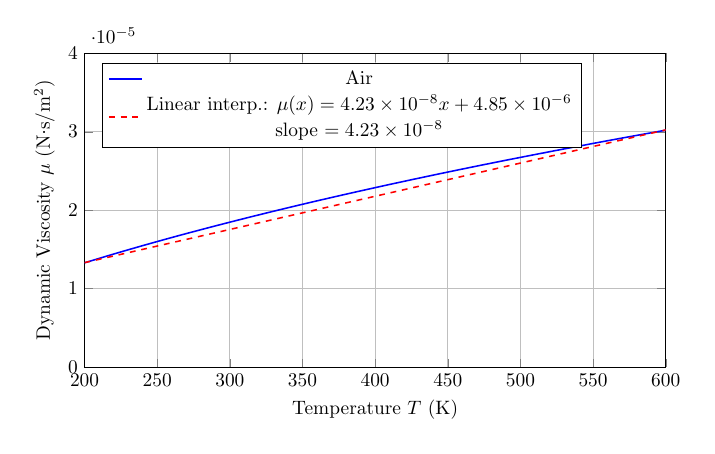
\begin{tikzpicture}[scale=0.7]
        \begin{axis}[
            width=\textwidth,
            height=0.6\textwidth,
            xlabel={Temperature $T$ (K)},
            ylabel={Dynamic Viscosity $\mu$ (N·s/m$^2$)},
            xmin=200, xmax=600,
            ymin=0, ymax=4e-5,
            domain=200:600,
            grid=both,
            legend pos=north west,
        ]
            % Sutherland's formula for Air
            \addplot [
                thick,
                blue,
                samples=200
            ]
            {(1.716e-5) * (x/273)^(3/2) * (273+111)/(x+111)};
            \addlegendentry{Air}

            % Linear interpolation of the above function (dashed red)
            \addplot [
                thick,
                dashed,
                red
            ]
            {(4.23e-8)*x + 4.85e-6};
            \addlegendentry{\shortstack{Linear interp.: $\mu(x)=4.23\times10^{-8}x+4.85\times10^{-6}$\\ slope $=4.23\times10^{-8}$}}
        \end{axis}
    \end{tikzpicture}
\end{figure}
